\section*{Введение}

	\addcontentsline{toc}{section}{Введение}
	
	Согласно исследованию 2006 года около 30 процентов звезд, принадлежащих нашей Галактике, находятся в составе, так называемых кратных систем, конкретнее двойных~\cite{charlesj.lada}. Двойная система представляет собой две звезды, вращающиеся вокруг общего центра масс, причем необязательно звезды по массам (и соответсвенно по размерам) являются одинаковыми. Хорошим и известным всем примером двойной системы является система Сириус, состоящая из белого карлика (Сириус B) и звезды главной последовательности Сириуса A. В двойной системе более массивная звезда эволюционирует быстрее и, в конечном счете, превращается в компактный объект, как например белый карлик, нейтронная звезда или черная дыра. Когда менее массивная звезда доходит до стадии расширения, в случае, если она находится достаточно близко к компактной звезде, ее внешние слои начинают перетекать на компактный компонент. Газ перетекает в аккреционный диск вокруг компактного компаньона, вращается, нагревается и в конце концов падает на компактную звезду. Кинетическая энергия аккрецируеммого вещества переходит в энергию излучения (при этом максимум интенсивности приходится на рентгеновский и мягкий гамма-диапазон). Изучение этого излучения может помочь понять свойства аккрецирующих объектов и механизмы генерации излучения.
	
	Граница между жестким ренгеновским и мягким гамма-излучением весьма условна. Оба вида излучения являются формами ионизирующего излучения (т.е. фотоны этих двух типов настолько высоко энергичны, что способны ионизировать атомы), но принято считать, что ренгеновское излучение имеет внеядерное происхождение, тогда как гамма --- результат изменения состояния ядер (будь-то их распад или слияние). Примерные границы ренгеновского излучения --- $0{,}1 - 300 $ КэВ, а гамма-излучения больше, чем $300$ КэВ.

	Нейтронные звезды --- звезды с очень малыми размерами (20-30 км в диаметре). Считается, что нейтронные звезды появляются в результате взрывов сверхновых. При взрыве происходит стремительный коллапс ядра нормальной звезды, которое затем и превращается в нейтронную звезду. Во время сжатия в силу закона сохранения момента импульса, а также сохранения магнитного потока происходит резкое увеличение скорости вращения и магнитного поля звезды. Высокая скорость вращения нейтронной звезды (она может достигать частоты около 100 оборотов в секунду) и чрезвычайно высокие магнитные поля ($10^{12} - 10^{13}$ Гс) являются основными условиями возникновения феномена рентгеновского пульсара. Хотя в начале нейтронные звезды в начале быстро вращаются, со временем они замедляются, поскольку излучают, ускоряют заряженные частицы и в следствие чего теряют часть своей энергии. Скорость вращения нейтронной звезды в итоге снижается настолько, что веществу ничего не препятствует падать на такую нейтронную звезду. Падая, вещество, уже будучи в состоянии плазмы, движется по линиям магнитного поля и ударяется о поверхность нейтронной звезды в районе её полюсов, разогреваясь до десятков миллионов градусов. Вещество, нагретое до столь высоких температур, ярко светится в рентгеновском диапазоне. Область, в которой происходит столкновение падающего вещества с поверхностью тела нейтронной звезды, очень мала — всего около 100 метров. Это горячее пятно из-за вращения звезды периодически пропадает из вида, поэтому наблюдаются регулярные пульсации рентген-излучения. Такие объекты и называются аккрецирующими рентгеновскими пульсарами.
	
	В черных дырах также возможны рентгеновские пульсации, хотя в них излучает сам аккреционный диск, разогретый до высоких температур. Разогрет он по причине того, что сама черная дыра является еще более компактным объектом по сравнению с нейтронной звездой, что делает аккреционный диск более плотным, а плазму более горячей, за счет столкновений.
	
	В космосе существуют тесные двойные системы, состоящие из компактного объекта (черной дыры или нейтронной звезды) и звезды-компаньона. Они могут быть источниками пульсирующего рентгеновского и мягкого гамма-излучения, которое может быть зарегистрировано различными космическими приборами (INTEGRAL, Swift/BAT, Konus-Wind и другие).
	
	Тесные двойные системы играют ключевую роль в понимании процессов аккреции и выбросов с компактных объектов в присутствии сильного магнитного и гравитационного поля, поэтому их изучение может помочь понять свойства аккрецирующих объектов и механизмы генерации излучения. Одним из представителей тесной двойной системы является кандидат в черную дыру MAXI J1820+070.
			
	Кандидат в черную дыру MAXI J1820+070 был впервые зарегистрирован 11 марта 2018 года с помощью прибора MAXI и был отождествлен с оптическим объектом ASASSN-18ey. Интенсивность источника достигла 3 Crab и её видимая звездная величина достигла значения $m_{V} = 12$ -- $13$. Столь яркое событие позволило наблюдать источник в различных диапазонах волн и различными космическими и наземными обсерваториями \cite{veledinaa.2018}. На рис. \ref{img:bh} представлена вспышка, которую зафиксировал прибор MAXI/GSC 10 марта 2018 года \cite{alert}.
	
	\begin{figure}[h!]
		\centering
			\begin{subfigure}[b]{0.49\linewidth}
			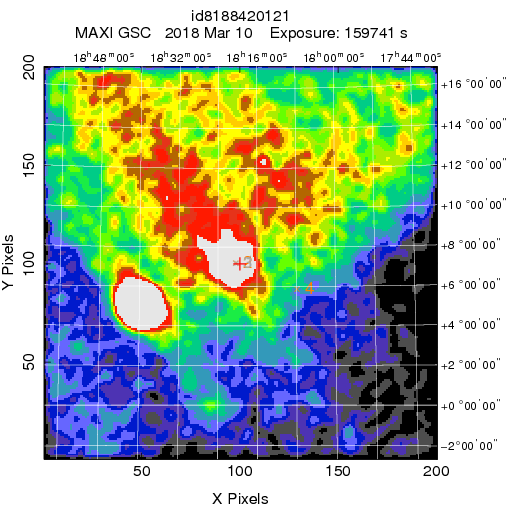
\includegraphics[width = \textwidth]{pictures/maxij_image_full.png}
			\caption{}
			\label{img:bhfull}
		\end{subfigure}
		\begin{subfigure}[b]{0.49\linewidth}
		\centering
			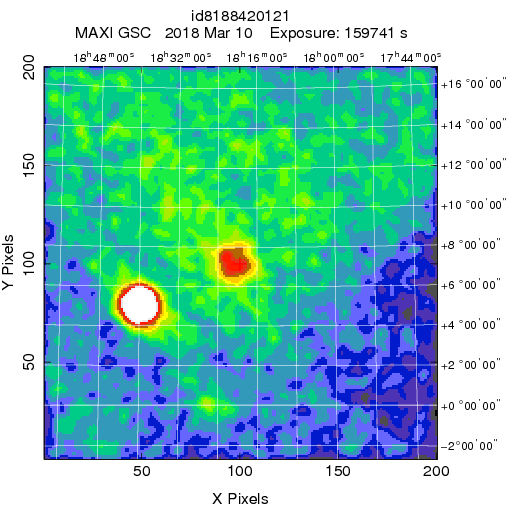
\includegraphics[width = \textwidth]{pictures/maxij_image.png}
			\caption{}
			\label{img:bhpart}
		\end{subfigure}
		\caption{Область неба, в которой был обнаружен MAXI J1820+070 в диапазоне от 2 до 20 кэВ (а) и диапазоне от 2 до 4 кэВ (b)}
		\label{img:bh}
	\end{figure}
	
	Квазипериодические колебания были в открыты в начале 80-х годах у нескольких маломассивных рентгеновских двойных. В отличие от периодического излучения, излучение этих объектов менялось в каких-то пределах: существенная часть излучения испытывала <<квазиколебания>> с <<квазипериодом>> от $\thicksim 0.1$ до $\thicksim 0.01$ Гц. Было предположено, что такие неустойчивые явления происходят при аккреции на нейтронные звезды, что хорошо согласовывалось с теоретическими моделями, но при дальнейшем изучении QPO были найдены и у кандидатов в черные дыры.
	
\section*{Научная новизна}
	
	В данной работе впервые произведен анализ излучения от аккрецирующей черной дыры (т.е. анализ ее спектра мощности и кривой блеска) по данным непрерывных наблюдений в течение порядка 190 дней в диапазоне энергий от $\sim13$ кэВ вплоть до $\sim300$ кэВ.
